
\subsubsection{Usability testing}
Based on Nielsen 2012 (https://medium.com/@iizzathisharah/the-five-usability-components-by-jakob-nielsen-detailed-insights-and-examples-90695af5ffb6)

\begin{itemize}
    \item learnability
    \item efficiency
    \item memorabiliy
    \item errors
    \item satisfaction
\end{itemize}
Magpie has remedied the first challenge of fragmented information on amenities. We will now address the second challenge: making the access to this information easy, quick \& accessible.\\

\noindent The goal of the user evaluation is to gain feedback from real users, learn if Magpie works as expected and assess overall user interface. Our approach is as follows:
%user evaluation approach
\begin{enumerate}
    \item Round up users from the market research + seek out others
    \item Conduct online usability sessions to discuss Magpie, explore the features, gather feedback,
    \item Synthesize notes from sessions and summarize points to improve
    \item Iteratively implement/improve features
\end{enumerate}
We interviewed 11 users in total. Some have decided to remain anonymous, therefore have been labelled as \emph{Anonymous n°}, while others will be referred to by their name. \\ They have been divided into the following categories: 6 general users, 3 targeted users, 1 UI/UX expert and 1 accessibility expert.\\
\emph{General users} are defined as those who use Magpie casually for personal interests.\\ \emph{Targeted users} are defined as those who use Magpie as a tool for their work.

\noindent Both controlled \& uncontrolled approaches were used for the sessions.\\
The controlled sessions were based around a strict list of tasks the user would complete and used metrics such as time taken, difficulty and task success rate.\\
The uncontrolled sessions let the users freely roam the application while we observed their behaviour interacting with each element and initiate discussion to obtain feedback on features to improve.\\

\noindent A table with a list of general tasks is used to quantitatively evaluate each feature the user interacted with. Metrics measured are task difficulty and task success rate. The list of general tasks increased as the test sessions went on because new features were being added iteratively.\\
The difficulty of the task is related to its status and how much time a user spent on it. The status of a task can either be `complete', `pass', or `fail' where:
\begin{itemize}
    \item \emph{complete} is attributed when the user completes the task on their own
    \item \emph{pass} is attributed when the user was able to complete the task but with our help
    \item \emph{fail} is attributed when the user was not able to complete the task even with our help
\end{itemize}
Lastly, a short satisfaction survey is administered at the end of each session quantify user experience and provide a baseline for improvements. User behaviour is also observed during the session to complement these quantitative metrics.\\
%figure for satisfaction survey
\begin{figure}[h!]
    \centering
    \fbox{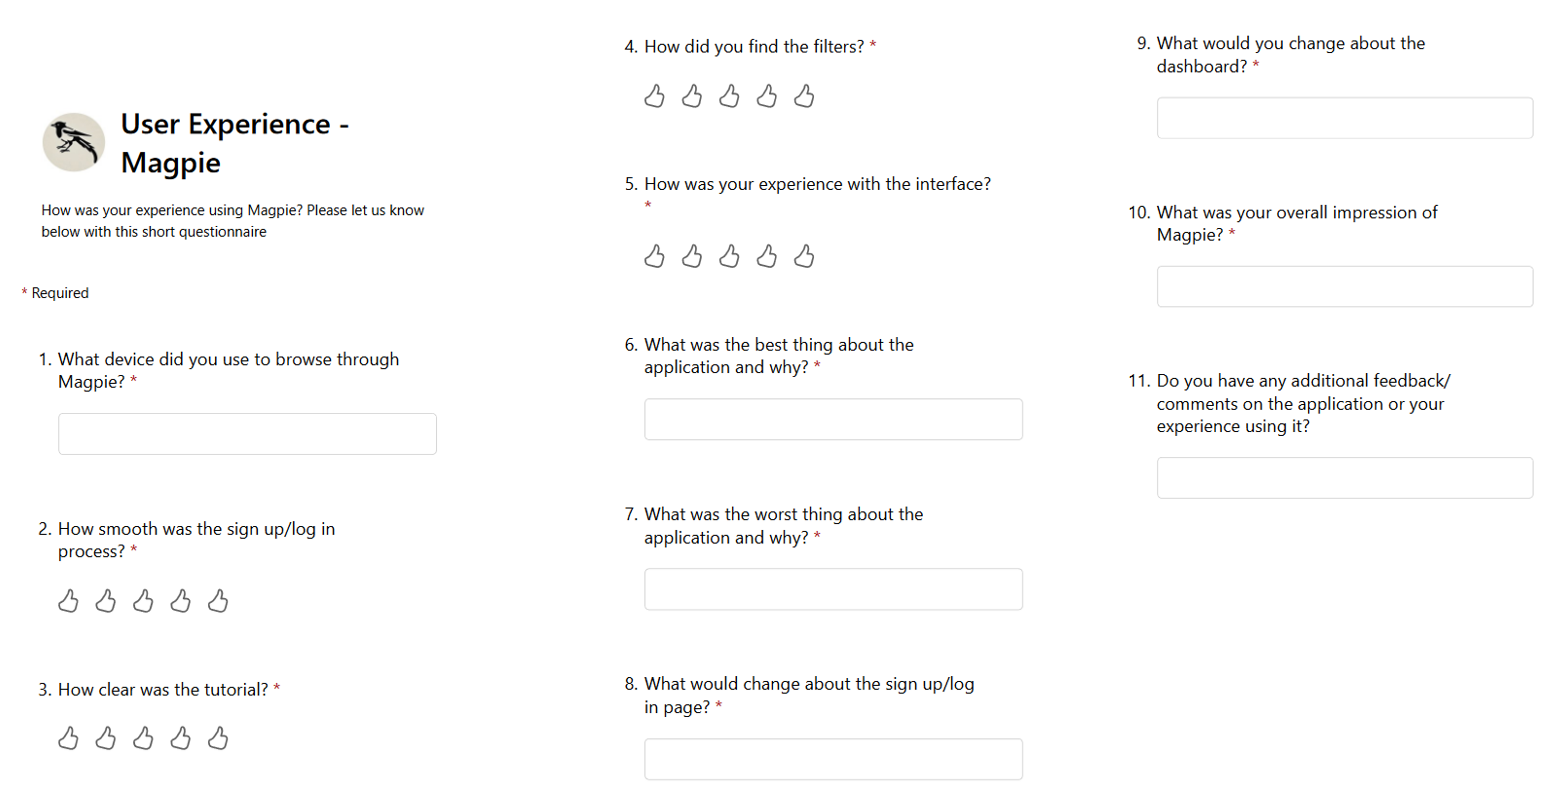
\includegraphics[width=0.7\textwidth]{images/user-satisfaction-survey.png}}
    \caption{User Evaluation - Satisfaction survey questions}
\end{figure}\\
The evaluation of Magpie has been divided into the following sections:
\begin{enumerate}
    \item General users test sessions
    \item Targeted users test sessions
    \item UX/UI expert review
    \item Accessibility expert review
\end{enumerate}
